\chapter{Project: the Kramers-Kronig receiver}
\label{h:kk-receiver}

\begin{quote}
The enormous advance in electronic technologies produced a new paradigm, where the detected photocurrent can be sampled and digitized, allowing all processing to be conducted in the digital domain. This situation gives access to an almost unlimited plethora of linear and nonlinear manipulations that can be applied to the photodetected signal.

--- Antonio Mecozzi
\end{quote}


\chaptertoc

In this chapter, we will combine the Kramers-Kronig relationships with a few new mathematical concepts and show how we can build a receiver that in some circumstances can reconstruct the phase of the signal from just a single amplitude measurement. This so-called Kramers-Kronig (KK) receiver was introduced in 2016 by Mecozzi \emph{et al.} and the approach we will follow here is based on one of their later review papers\footnote{Mecozzi \emph{et al.}, Adv. Opt. Photon., 11, 3, 480, 2019.}.

First, we will give a brief primer on optical coherent communications, and show how telecom signals are typically represented and detected, and what problems can arise.

Next, we will see under what circumstances the phase of a signal can be derived from a single amplitude measurement. We will introduce concepts from complex analysis like winding numbers, logarithmic derivatives and the argument principle.

Finally, we will combine this with the Kramers-Kronig relations to construct the complete KK receiver algorithm.

\pagebreak

\section{Coherent optical communications}

Let's say we have an information signal $a_s(t)$ (real-valued) that we want to transmit using an optical link. However, the frequencies of light waves used for communication are hundreds of THz, typically orders of magnitude higher than the frequencies contained in the information signal $a_s(t)$. To solve this frequency mismatch, we will use $a_s(t)$ to modulate the amplitude of an optical carrier wave with angular frequency $\omega_0$. This gives rise to the following electric field $E(t)$:

\begin{equation}
E(t) = a_s(t) \cos(\omega_0 t)
\end{equation}

Now suppose we additionally want to encode information in the phase $\phi_s(t)$ of the optical signal. Since the phase of the optical carrier needs to be well-defined and stable for that, this requires coherent sources, and we talk about \textbf{coherent optical communication}. Using this approach, the electric field we are transmitting becomes

\begin{equation}
 E(t) = a_s(t) \cos\left(\omega_0 t + \phi_s(t)\right)  
 \label{eq-electric-field-modulated} 
\end{equation}

\begin{cue}
If you measure this signal with a photodiode, what signal do you get? Can you recover all information?  
\end{cue}
    
The photocurrent measured at the output of the photodiode will be proportional to

\begin{align}
 E(t)^2 &= a_s^2(t) \cos^2\left(\omega_0 t + \phi_s(t)\right) \nonumber \\
 &= \frac{a_s^2(t)}{2} \left[ 1 + \cos\left(2\omega_0 t + 2\phi_s(t)\right)\right]  
 \label{eq-photocurrent-detected}
\end{align}

However, remember that $\omega_0$ (and obviously also $2\omega_0$) is an insanely high frequency for our photodiode, way too high to be measured. Therefore, the measured signal will only contain the first term, containing the square of the amplitude modulation $a_s(t)$. Unfortunately, this means that we have lost all the information encoded in $\phi_s(t)$, which is clearly a problem that needs solving.
    
\begin{cue}
Would this also be an issue if we were working with radio waves instead of light?  
\end{cue}
    
Radio waves are much lower in frequency, and are detected using an antenna, where the electric field directly drives the motion of the electrons in a metal conductor. In this way, the phase of the electromagnetic wave (i.e. at what time it becomes zero or maximal) is imprinted on the time evolution of the antenna current. So, provided the modulation and the carrier frequency are not too fast, this phase can be measured directly, by looking at when the current becomes zero or maximal.

Going back to optical communications, there exist a number of techniques to recover both the amplitude and the phase from one or more intensity measurements. They all have in common that they construct a new signal, which is the sum of the signal carrying the actual information, and a reference signal, which is an unmodulated tone at a reference frequency $\omega_\mathrm{ref}$:

\begin{equation}
E(t) = A_\mathrm{ref} \cos\left(\omega_\mathrm{ref} t + \phi_\mathrm{ref}\right) + a_s(t) \cos\left(\omega_0 t + \phi_s(t)\right)  
\end{equation}

This reference tone can either be added at the source or at the detector of the optical link.

If $\omega_\mathrm{ref} = \omega_0$, we are talking about \textbf{homodyne detection} schemes. If the carrier frequency is different from the reference frequency, we are dealing with \textbf{heterodyne detection}.

A classical way of recovering both amplitude and phase would be to perform two amplitude measurements in a homodyne scheme, with two reference tones that are 90 degrees out-of-phase with respect to each other. We will not be discussing the mathematics of how exactly this works, but only mention that a drawback of this scheme is that it requires four separate photodiodes.

One of the goals of the Kramers-Kronig receiver is to have a much simpler (and therefore potentially cheaper) scheme which requires only a single photodiode. The price we will pay for this, as we shall see, is more processing in the digital domain after the detector.


\pagebreak

\section{Complex envelope}

In what follows, it will be useful to work with a frequency-domain representation of the signals.

\begin{cue}
Using the phasor concept from Section~\ref{s:phasor}, what is the phasor associated with $E(t)$ in Eq.~\ref{eq-electric-field-modulated}, and how do you recover the full time-varying signal $E(t)$ from it?    
\end{cue}

We can define a complex number $\tilde{a}_s(t)=a_s(t) \exp(j \phi_s(t))$,
and $E(t)$ can be recovered from it as

\begin{equation}
E(t) = \Re \left(\tilde{a}_s(t) e^{j \omega_0 t}\right) = \Re \left(a_s(t) e^{j \left(\omega_0 t + \phi_s(t)\right)}\right)
\end{equation}

\noindent\marginnote[-1.8cm]{As before, we choose to use $e^{j \omega t}$ rather than $e^{-j \omega t}$ as time dependence, but be aware that other people make different choices.}So, $\tilde{a}_s(t)$ can be seen as the phasor associated to $E(t)$. (The difference compared to Section~\ref{s:phasor} is that now this phasor is time-dependent.) 

Another name for this phasor is the \textbf{complex envelope} or the \textbf{complex amplitude} of the transmitted signal.

\begin{cue}
What is the relationship between the complex amplitude and the time-varying photocurrent that we get out of a photodiode detecting $ E(t) = a_s(t) \cos\left(\omega_0 t + \phi_s(t)\right) $?  
\end{cue}

Looking back at Eq.~\ref{eq-photocurrent-detected}, and taking into account the bandwidth limitations of the detector, the photocurrent is proportional to

\begin{equation}
\frac{a_s^2(t)}{2} = \frac {\left| \tilde{a}_s(t) \right|^2}{2}
\end{equation}

Since there are already other proportionality constants when relating the square of the electric field to the photocurrent (i.e. the responsivity of the photodiode), we will typically also sweep the factor $\frac{1}{2}$ under the rug and only look at the squared magnitude of the complex envelope.

\begin{cue}
What would be the complex envelopes of the signals used for homodyne and heterodyne detection?      
\end{cue}

For homodyne detection, note that the real part of a sum is equal to the sum of the real parts. This means that also the phasor of the sum of signals is the sum of the corresponding phasors:

\begin{equation}
\tilde{a}(t) = A_\mathrm{ref} e^{j \phi_\mathrm{ref}} + a_s(t) e^{j \phi_s(t)} =  \tilde{A}_\mathrm{ref} + \tilde{a}_s(t)
\end{equation}

In the heterodyne case, we have

\begin{align}
\tilde{a}(t) &=  A_\mathrm{ref} e^{j \phi_\mathrm{ref}} e^{-j ( \omega_0 - \omega_\mathrm{ref} ) t } + a_s(t) e^{j \phi_s(t)} \noref \\
   &= \tilde{A}_\mathrm{ref} e^{-j ( \omega_0 - \omega_\mathrm{ref} ) t } + \tilde{a}_s(t)
\end{align}

Indeed, focusing only on the essential bits, and not worrying about amplitudes and phases for the moment, we have

\begin{equation}
\Re \left( e^{-j (\omega_0 - \omega_\mathrm{ref})t }  e^{j \omega_0 t} \right) = \Re \left( e^{j \omega_\mathrm{ref}t \right) = \cos{ \left( \omega_\mathrm{ref}t \right)}
\end{equation}

From now on, we will only work with complex amplitudes. To make our notational life a bit easier, we will omit the tilde that stresses that we are dealing with phasors, and just write e.g. for the homodyne case that $a(t) = A_\mathrm{ref} + a_s(t)$, where all terms are implied to be complex-valued phasors.

\hl{TODO: Jupyter notebook}

\pagebreak

\section{Single-sideband signals}

\noindent\marginnote{Some people mean something slightly different by SSB: not a complex-valued signal to the right of a carrier, but a real-valued signal where the sideband has been removed.}For the Kramers-Kronig receiver, we will restrict ourselves to a specific subset of signals. Indeed, we will assume that the frequency content of the complex-valued information envelope $a_s(t)$ is entirely to the right of the reference signal. Let's call such a signal a \textbf{single-sideband (SSB)} signal. In this content, the reference signal is sometimes also called the \textbf{subcarrier}.

In what follows, let's modify our signals by shifting the frequency axis from $f$ to $f'$ such that $f_\mathrm{ref}$ (and $\omega_\mathrm{ref}$ for that matter) become zero (Fig.~\ref{fig-ssb}). The original signals can easily be recovered by shifting the frequencies back, but this notational trick makes the formulas more compact, looking a bit like homodyne detection.

\begin{marginfigure}[-2.0cm]
    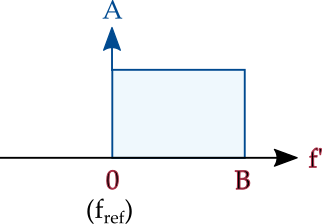
\includegraphics{kk/figures/SSB}
    \caption{A single-sideband signal. Note that there are no frequencies to the left of $f'=0$.}
    \label{fig-ssb}
\end{marginfigure}

Let's also assume that $a_s(t)$ has a finite frequency spectrum that is contained in the range $]0, B]$ on the shifted axis (i.e., angular frequencies in the range $]0, 2\pi B]$). 

In summary, we can write the complex envelope of an SSB signal as $a(t) = A + a_s(t)$, with the complex phasor $a_s(t)$ being bandlimited and containing only positive (angular) frequencies.

\begin{cue}
What do you get when you detect such a signal with a photodiode?
\end{cue}

The photocurrent is proportional to

\begin{align}
\left| a(t) \right| ^2 =&  \left(A + a_s(t) \right) \left(A^* + a_s^*(t) \right) \nonumber \\
 =& |A|^2 + \left| a_s(t) \right|^2 + Aa_s^*(t) + A^*a_s(t)  \nonumber \\
 =& |A|^2 + \left| a_s(t) \right|^2 + 2 \Re \left(A^* a_s(t) \right)
\end{align}

\begin{cue}
Without loss of generality, put the phase of $A$ to zero and simplify.
\end{cue}

We get 
\begin{equation}
\left| a(t) \right| ^2 = A^2 + \left| a_s(t) \right|^2 + 2 A \Re \left(a_s(t) \right)
\label{eq-kk-heterodyne}
\end{equation}

At first, it seems hopeless to extract both the amplitude and the phase of $a_s(t)$ from this measurement. Even if we assume that the amplitude $A$ of the subcarrier is known (e.g. because we've added it ourselves at the detector), there are still a lot of terms which mix different pieces of information. However, before we're able to solve this, we need to lay some more groundwork first.

\pagebreak

\begin{exer}
% difficulty: normal
By making use of the definition of the Fourier transform 

$$\tilde{x}(\omega) = \int_{-\infty}^{\infty}x(t) e^{-j \omega t} dt$$

and the conjugate of that expression, show that if $a_s(t)$ only contains positive frequencies, then $a_s^*(t)$ contains only negative frequencies. For such signals, would knowing $\Re \left(a_s(t) \right)$ be enough to fully reconstruct $a_s(t)$?
\end{exer}

\iffalse

In general, just knowing $\Re \left(a_s(t) \right)$ would not be enough to figure out both amplitude and phase separately. However, don't forget that we are dealing with SSB signals here.

Since

$$\Re \left(a_s(t) \right) = \frac{1}{2}\left(a_s(t) + a_s^*(t) \right)$$

and since for SSB signals, $a_s(t)$ + $a_s^*(t)$ do not overlap in frequency, can just keep only the positive frequencies from $\Re \left(a_s(t) \right)$ and completely recover $a_s(t)$ that way.

\fi

\pagebreak

\section{Z-extension}

\subsection{Definition}

When we will perform digital signal processing on the detected signal, we will do so chunk-by-chunk, i.e. at any one time only working with a signal of finite length $T$. Let's now periodically extend this signal, such that $a(t)$ becomes a signal with period $T$.

\begin{cue}
Using all the assumptions we have made so far for our signal $a(t)$, write down its Fourier series.
\end{cue}

In general, the Fourier series of a periodic signal $a(t)$ is given by

\begin{equation}
a(t) = \sum_{k=-\infty}^\infty a_k e^{jk\Omega t}
\end{equation}

\noindent\marginnote{It's important to realise that $\Omega$ has nothing to do with the carrier frequency, but is only related to the duration of the chunk!}Here, $\Omega=2 \pi / T$, i.e. the angular frequency related to the duration of the chunk that we will process.

The Fourier coefficients $a_k$ satisfy

\begin{equation}
a_k = \frac{1}{T} \int_0^T a(t) e ^{-jk\Omega t} dt
\end{equation}
    
However, our signal has certain restrictions. First of all, we know that the maximum frequency $f$ in $a(t)$ is equal to $B$. Let's assume that $B$ is an integer multiple of $1/T$ (an approximation which becomes easier the larger $T$ becomes). If $B=M/T$,  with $M$ an integer, then the largest angular frequency $\omega$ becomes $2 \pi M/T = M \Omega$. Also, remember that because $a(t)$ is single-side band, it has no negative frequencies.

\begin{cue}
Combine all of this to get the final Fourier representation of $a(t)$. Which component corresponds to the subcarrier $A$?
\end{cue}

Finally, we get

\begin{equation}
a(t) = \sum_{k=0}^M a_k e^{jk\Omega t}
\label{eq-a-fourier}
\end{equation}

Here, $a_0$ corresponds to our subcarrier $A$.

\begin{cue}
Transform this Fourier representation into a complex-valued expression by using the substitution $z=e^{j\Omega t}$.
\end{cue}

\noindent\marginnote{Astute readers might identify this as the Z-transform of the reversed sequence of Fourier coefficients $a_k$.}This results in the following polynomial, which Mecozzi called the \textbf{Z-extension} of $a(t)$:

\begin{equation}
\mathcal{Z}_a(z) = \sum_{k=0}^{M} a_k z^k
\end{equation}

By construction, if we evaluate the Z-extension for $z=e^{j\Omega t}$, we recover the original signal $a(t)$:

\begin{equation}
\mathcal{Z}_a\left(e^{j\Omega t}\right) = \sum_{k=0}^{M} a_k e^{j k \Omega t} = a(t)
\label{eq-z-a-recovery}
\end{equation}

Since the Z-extension is a complex polynomial of order $M$, we know that it has $M$ zeroes, which we will call $z_k$. This means we can also write the Z-extension as

\begin{equation}
\mathcal{Z}_a(z) = a_M \prod_{k=1}^{M} (z-z_k)
\label{eq-z-ext-factorisation}
\end{equation}

So, if we know the zeroes $z_k$, then we can construct the Z-extension, at least up to an irrelevant scaling factor. Then, by evaluating this Z-extension on the unit circle, we can recover the original signal $a(t)$. 

So, \emph{apart from a scaling factor, the location of the zeroes $z_k$ of the Z-extension $\mathcal{Z}_a(z)$ uniquely determines $a(t)$}.

\begin{exer}
% difficulty: trivial 
Write $a_M$ as a function of the carrier amplitude $A$ and the zeroes $z_k$.
\begin{sol}
A = a_0 = a_M \prod_{k=1}^{M} (-z_k)
\end{sol}

\end{exer} 

\pagebreak

\subsection{Z-extension of $a^*(t)$}

\begin{cue}
By taking the complex conjugate of the Fourier representation of $a(t)$, derive $\mathcal{Z}_{a^*}(z)$, the Z-extension of $a^*(t)$.
\end{cue}

Start from Eq.~\ref{eq-a-fourier}:

\begin{equation}
a(t) = \sum_{k=0}^M a_k e^{jk\Omega t}
\end{equation}

Taking the complex conjugate, we get

\begin{equation}
a^*(t) = \sum_{k=0}^M a_k^* e^{-jk\Omega t}
\end{equation}

By definition, we get the Z-extension of a signal by the substitution $z=e^{j\Omega t}$ in its Fourier series. This gives us

\begin{equation}
\mathcal{Z}_{a^*}(z) = \sum_{k=0}^M a_k^* z^{-k}
\end{equation}

So, this time, the Z-extension has only negative powers, corresponding to negative frequencies.

Let's now compare this with the Z-extension of $a(t)$:

\begin{equation}
\mathcal{Z}_a(z) = \sum_{k=0}^{M} a_k z^k
\end{equation}

\begin{cue}
Show that $\left[\mathcal{Z}_a\left(\frac{1}{z^*}\right)\right]^* = \mathcal{Z}_{a^*}(z)$
\end{cue}
    
Indeed, 

\begin{align}
    \left[\mathcal{Z}_a\left(\frac{1}{z^*}\right)\right]^* =& \left[ \sum_{k=0}^{M} a_k \left(\frac{1}{z^*}\right)^k \right]^* \nonumber \\
    =& \sum_{k=0}^{M} a_k^* z^{-k} \nonumber \\
    =& \ \mathcal{Z}_{a^*}(z)
    \label{eq-zeroes-z-ext}
\end{align}

This relation is true for all possible $z$, so it will certainly be true if $z$ is a zero of $\mathcal{Z}_{a^*}$. Therefore, from putting Eq.~\ref{eq-zeroes-z-ext} to 0, we get that \emph{the zeroes of the Z-extension of $a^*(t)$ are the inverse conjugates of the zeroes of the Z-extension of $a(t)$. }

\begin{cue}
Factor $\mathcal{Z}_{a^*}(z)$ using its roots.
\end{cue}

Let's start from the factorisation Eq.~\ref{eq-z-ext-factorisation}:

\begin{equation}
\mathcal{Z}_a(z) = a_M \prod_{k=1}^{M} (z-z_k)
\end{equation}

Using the relationship  $\mathcal{Z}_{a^*}(z) = \left[\mathcal{Z}_a\left(\frac{1}{z^*}\right)\right]^*$, we get

\begin{align}
    \mathcal{Z}_{a^*}(z) =& \left[ a_M \prod_{k=1}^{M} \left(\frac{1}{z^*}-z_k \right) \right]^* \nonumber \\
    =& \ a_M^* \prod_{k=1}^{M} \left(\frac{1}{z}-z_k^* \right) \nonumber \\
    =& \ \frac{a_M^*}{z^M} \prod_{k=1}^{M} \left(1 - z_k^* z \right) \nonumber \\
    =& \ \frac{a_M^*}{z^M} \prod_{k=1}^{M} z_k^* \left(\frac{1}{z_k^*} - z \right) 
\end{align}

Note that this time we not only have $M$ zeroes, we also have a pole of order $M$ at the origin.

\begin{cue}
What can you say about $z_k$ and $1/z_k^*$ in terms of their position with respect to the unit circle?
\end{cue}

Because they have amplitudes $|z_k|$ and $|1/z_k|$, one of these zeroes will be inside the unit circle, while the other one will be outside. Remember this, as this will become important later on!

\pagebreak

\subsection{Z-extension of $|a(t)|^2$}

\begin{cue}
Knowing what you know now, derive the Z-extension of the intensity $|a(t)|^2$, which is simply $a(t)a^*(t)$.
\end{cue}

As usual, we start from a representation in Fourier space:

\begin{equation}
|a(t)|^2 = \left[  \sum_{k=0}^M a_k e^{jk\Omega t} \right] \cdot \left[ \sum_{k'=0}^M a_{k'}^* e^{-jk'\Omega t}\right]     
\end{equation}

To arrive at the Z-extension, we need to perform the substitution $z=e^{j\Omega t}$, so the Z-extension of $|a(t)|^2$ is just the product of the Z-extensions of $a(t)$ and of $a^*(t)$:

\begin{equation}
\mathcal{Z}_{|a|^2}(z) = \mathcal{Z}_a(z) \mathcal{Z}_{a^*}(z)
\end{equation}

At this point, you might be forgiven for wondering what the point of all of this is, especially since our original goal is to determine under which circumstances we can unambiguously determine the phase of a signal from a measurement of its amplitude. However, at this stage, we have all the tools in hand to take the next step in answering that question.

\pagebreak

\section{Minimum-phase signals}

Let's repeat what we've learned so far. Apart from an irrelevant scaling factor, the time dependence of the bandlimited SSB signals $a(t)$ we have been studying, is uniquely determined by the location of the $M$ zeroes of their Z-extension. However, what we detect with our photodiode is not $a(t)$, but rather $|a(t)|^2$, of which the time evolution is determined by the location of the $2M$ zeroes of its Z-extension. These zeroes come in pairs, $z_k$ and $1/z_k^*$, one of which pertains to $a(t)$ and the other one to $a^*(t)$.

\begin{cue}
Starting from a certain signal $a(t)$ and the zeroes of its Z-extension, how can you construct a new signal $a'(t)$ with the same intensity $|a(t)|^2=|a'(t)|^2$?   
\end{cue}

Focus e.g. on a certain zero $z_k$ of the Z-extension of $a(t)$. As we know, $1/z_k^*$ will be a zero of the Z-extension of $a^*(t)$. Let's now create a new complex signal $a'(t)$ by replacing the zero $z_k$ by $1/z_k^*$. Even though this results in a different signal $a'(t)$, the entire set of zeroes of the Z-extension of $|a'(t)|^2$ will still be the same as the original set of zeroes of the Z-extension of $|a(t)|^2$. As such, the time evolution of the intensity has not changed. The only thing that has changed is which zeroes belong to $a(t)$ and which to $a^*(t)$.

\begin{cue}
What is the upper bound on the number of different signals you can construct which have the same intensity? Why is this an upper bound and not an exact value?   
\end{cue}

Look at the set of zero pairs of $\mathcal{Z}_{|a|^2}(z)$. For each of these $M$ pairs, we have two possibilities, assigning one of the zeroes to either $\mathcal{Z}_{a}(z)$ or to $\mathcal{Z}_{a^*}(z)$. So, there's a maximum of $2^M$ variations in total. Not all of these need to result in different signals. E.g., a zero could lie on the unit circle, so that $z=1/z^*$, and exchanging them does not matter. Or the same pair of zeroes could appear more than once, such that we don't have $M$ distinct zero pairs.

In any case, if we measure the intensity $|a(t)|^2$ of the signal at the receiver, we don't know which of $\le2^M$ signals $a(t)$ the sender intended to communicate to us. However, we could all agree to follow a certain convention when transmitting signals. 

\pagebreak

For that purpose, it's important to remember that in a pair of zeroes $(z, 1/z^*)$, one lies inside the unit circle and the other one outside. Let's e.g. decide that we will only use signals $a(t)$ where the zeroes lie outside of the unit circle. In that way, we have lifted all ambiguity, since there is only one way to partition the zeroes of the Z-extension of $|a(t)|^2$ into a group related to $a(t)$ and another related to $a^*(t)$.

Such signals are called \textbf{minimum-phase signals}. However, one question still remains. How can we make sure that a minimum-phase signal at the transmitter will still be minimum-phase after travelling through a distorting fibre? To achieve this, we need some more concepts from complex analysis. This will also give us more insight into the nature of minimum-phase signals, and will also allow us to explain why they are called that way.

\pagebreak

\section{Winding number}

Suppose we have a closed path in the complex plane, and we want to express how many times this path encircles a certain point. We define this \textbf{winding number} to be positive if the turns are in the counterclockwise direction.

\begin{cue}
Draw some paths with positive, negative and zero winding numbers.    
\end{cue}

Fig.~\ref{fig-winding} shows a number of paths around a certain point, indicated by the black dot, and their corresponding winding numbers.

\begin{figure}[h]
% credits: Wikipedia
\centering
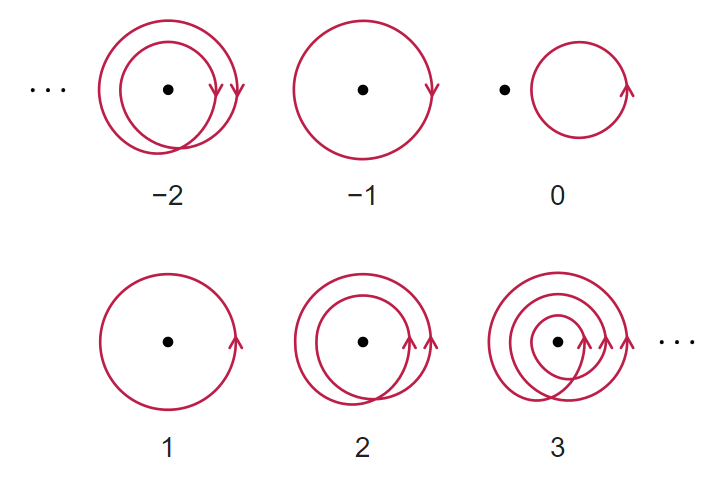
\includegraphics[width=8cm]{kk/figures/winding_number}
\caption{Paths with different winding numbers around the black dot.}
\label{fig-winding}
\end{figure}

Note that if a path does not encircle the point, then its winding number around that point is zero.

\begin{exer}

% difficulty: trivial
What is the winding number of $C$ around $p$?

\begin{center}
% credits: Wikipedia
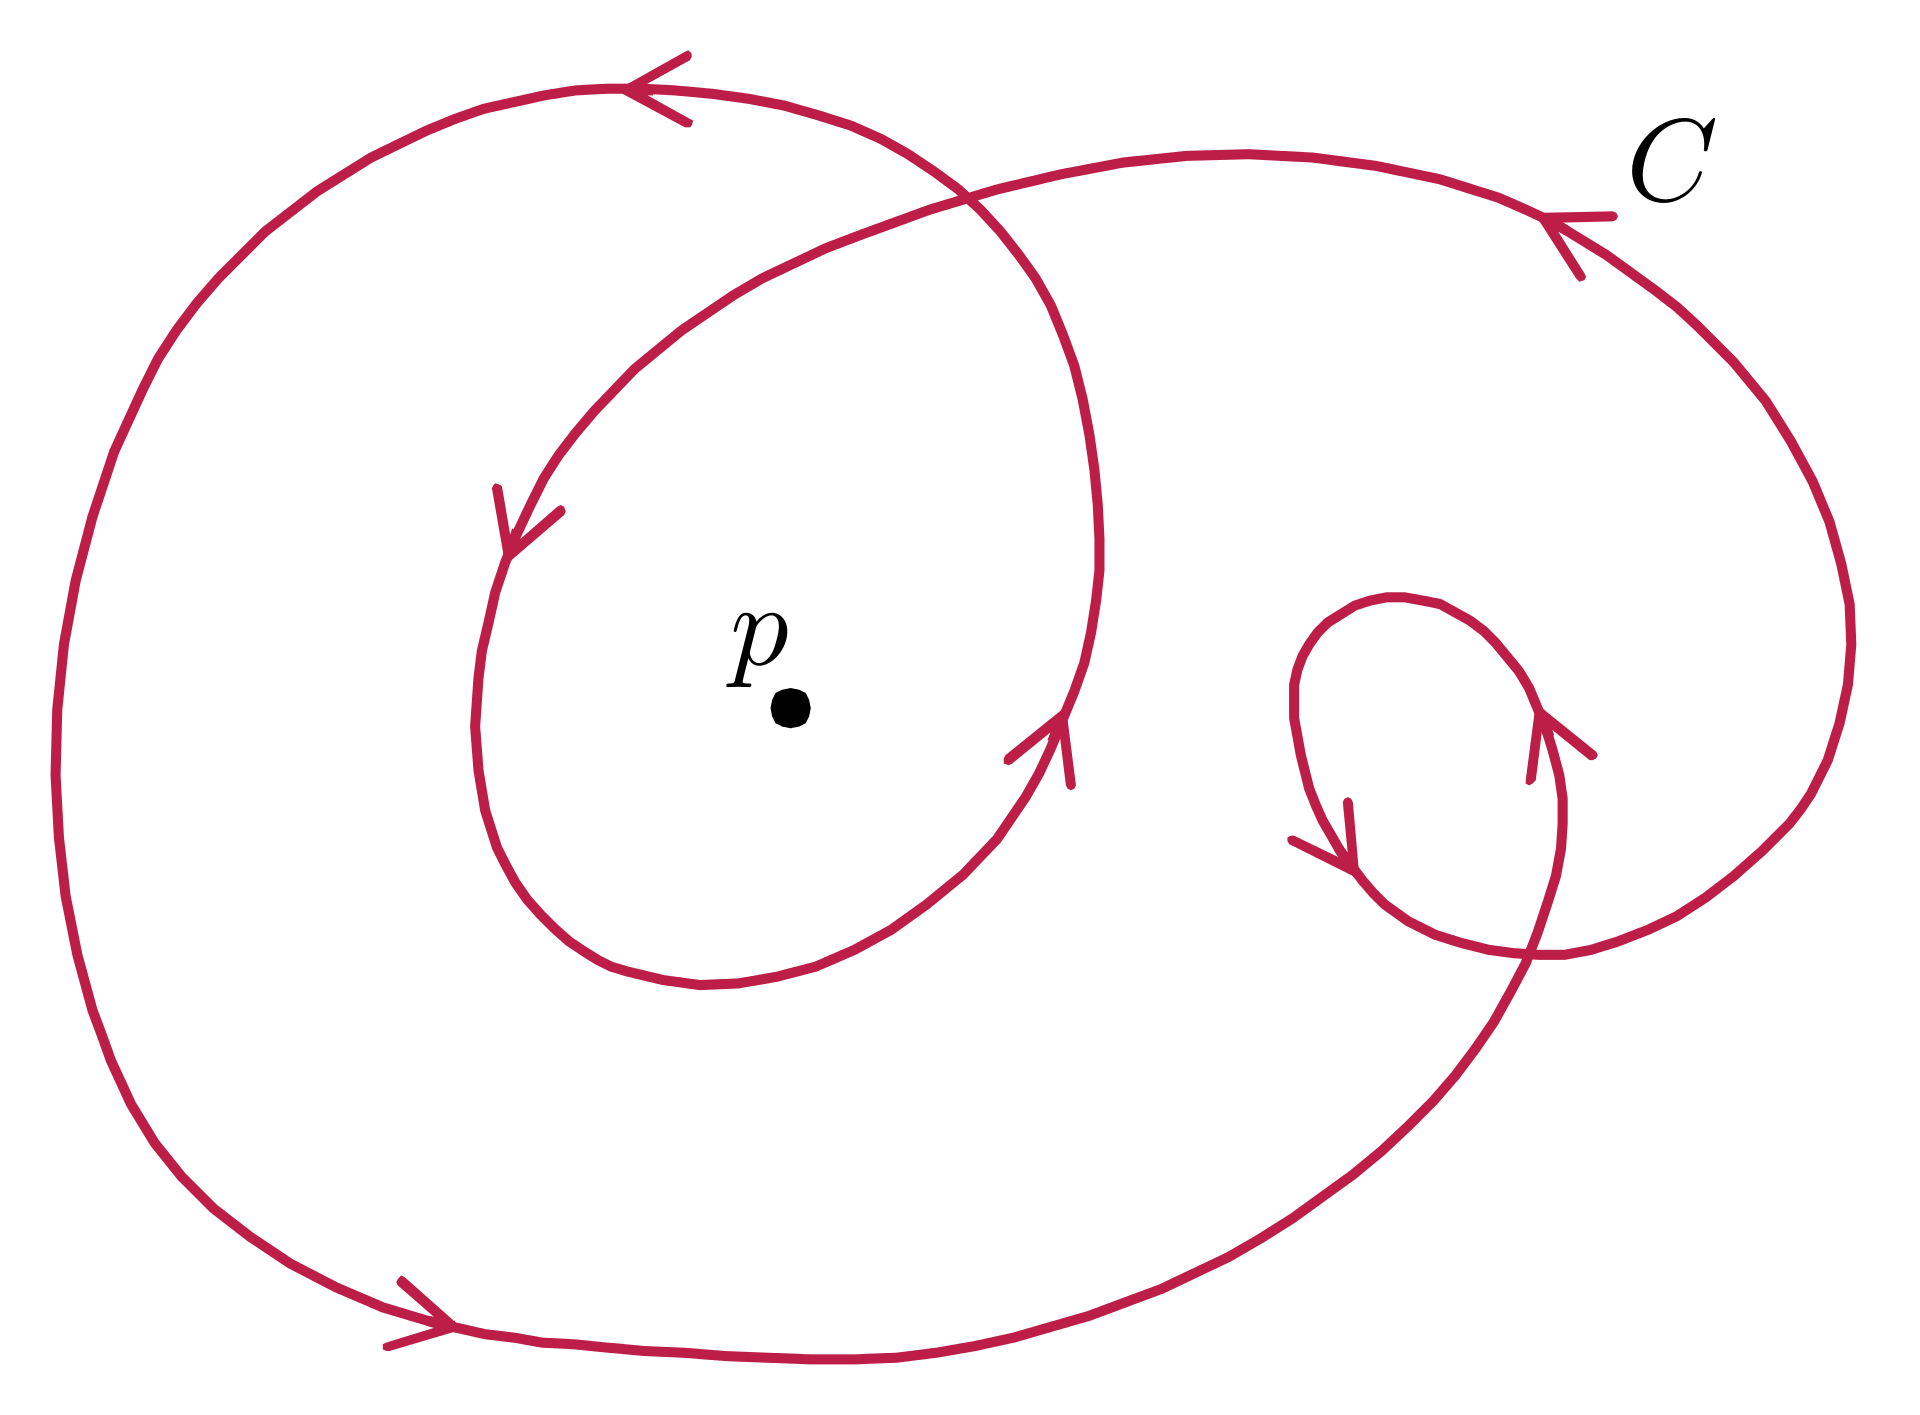
\includegraphics[width=4cm]{kk/figures/winding_number_exer}
\end{center}

\begin{sol}
2
\end{sol}

\end{exer}

Since $C$ is a closed contour, we could wonder whether there is an integral of a certain function over that contour which would give us the winding number.

\pagebreak

\begin{cue}
Express $dz/z$ in polar coordinates.    
\end{cue}

Starting from $z=r e^{j\theta}$, we have

\begin{equation}
dz = e^{j\theta} dr + jr  e^{j\theta} d \theta 
\end{equation}   

So

\begin{equation}
\frac{dz}{z} = \frac{dr}{r} + j d\theta = d [\ln r] + j d\theta    
\end{equation}

If we integrate $dz/z$ over a closed contour, the first term will vanish, since the beginning and the end point are the same, so that $\ln z$ will evaluate to the same number there. For the second term, we can't really use the same line of reasoning, as we will also require that the angle varies continuously throughout the contour. E.g., the angle at the start of the contour could be zero, while it could be $2 \pi$ at the end, indicating that we have taken one roundtrip around the origin. 

In any case, the integral of $dz/z$ will equal $j$ times the total change in angle when traversing the path. So, the winding number of a contour $C$ around the origin can be calculated as

\begin{equation}
\frac{1}{2 \pi j} \oint_C \frac{dz}{z}   
\end{equation}

\begin{exer}
% difficulty: trivial
Use Cauchy's formula to verify that the winding number around $z_0$ of a circle with centre at $z_0$ is indeed 1.
\end{exer}


\pagebreak

\section{Logarithmic derivative}

Just for fun, let's define the logarithmic derivate $\mathcal{L}(f(z))$ of the complex function $f(z)$ as

\begin{equation}
    \mathcal{L}(f(z)) \stackrel{def}{=} \frac{d}{dz}\ln\left(f(z)\right) = \frac{f'(z)}{f(z)}
\end{equation}

\begin{exer}
% difficulty: trivial
Show that for the logarithmic derivative similar properties hold as for the ordinary logarithm:

$$\mathcal{L}(f(z)g(z)) = \mathcal{L}(f(z)) + \mathcal{L}(g(z))$$

and

$$\mathcal{L}\left(\frac{f(z)}{g(z)}\right) = \mathcal{L}\left(f(z)\right) - \mathcal{L}(g(z))$$

\end{exer}

\pagebreak

\section{Argument principle}

Now we can play with our new toy and calculate the contour integral of the logarithmic derivative:

\begin{equation}
\oint_C \mathcal{L}(f(z)) dz = \oint_C \frac {d \ln\left(f(z)\right)} {dz} dz = \oint_C \frac{f'(z)}{f(z)} dz 
\end{equation}

\begin{marginfigure}[-1cm]
\centering
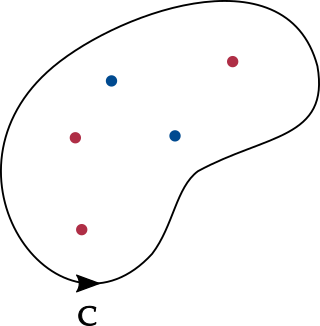
\includegraphics{kk/figures/arg_princ}
\caption{Contour which encloses $N=2$ (blue) zeroes and $P=3$ (red) poles of $f(z)$.}}
\label{fig-arg-princ}
\end{marginfigure}
Let's assume that the function $f(z)$ is holomorphic inside $C$, apart from $P$ poles. Let's also say that $f(z)$ has $N$ zeroes inside the contour (Fig.~\ref{fig-arg-princ}).

This means we can factor out the zeroes $z_k$ and the poles $p_j$, and write $f(z)$ as

\begin{equation}
f(z) = \frac{\prod_{k=1}^{N}\left(z-z_k\right)}{\prod_{j=1}^{P}\left(z-p_j\right)} g(z)
\end{equation}

Here, $g(z)$ is a holomorphic function without any zeroes inside $C$.

\begin{cue}
Using this factorisation, calculate $\mathcal{L}(f(z))$, based on the properties of logarithmic derivatives.
\end{cue}

We get

\begin{align}
\mathcal{L}(f(z)) &= \mathcal{L} \left(\prod_{k=1}^{N}\left(z-z_k\right)\right) - \mathcal{L} \left(\prod_{j=1}^{P}\left(z-p_j\right)\right) + \mathcal{L} (g(z)) \nonumber \\
&= \sum_{k=1}^{N}\frac{1}{z-z_k}-\sum_{j=1}^{P}\frac{1}{z-p_j} + \frac{g'(z)}{g(z)}
\end{align}

The integral will contain the sum of several contributions. As for the last term, since $g(z)$ has neither zeroes nor poles, $g'(z)/g(z)$ is holomorphic, and therefore that term vanishes because of Cauchy's theorem. As for integrals of terms like $1/(z-a)$, thanks to our expertise in complex analysis, we immediately know that those will result in $2 \pi j$ if $a$ is inside the contour. So finally

\begin{equation}
\fbox{$\displaystyle
\frac{1}{2 \pi j }\oint_C \frac{f'(z)}{f(z)} dz = N-P
$}
\label{eq-arg-princ}
\end{equation}

\pagebreak

Why is this called the argument principle? What is the relation with arguments (i.e. angles) of complex numbers?

\begin{cue}
Do a change of variables $w=f(z)$ and interpret the result.   
\end{cue}

Since $dw = f'(z) dz$, we get

\begin{equation}
\frac{1}{2 \pi j }\oint_C \frac{f'(z)}{f(z)} dz = \frac{1}{2 \pi j }\oint_{f(C)} \frac{dw}{w}
\label{eq-arg-principle-winding}
\end{equation}

\noindent\marginnote{Note that this is \textbf{not} the winding number of $C$ in the $z$-plane, but of $f(C)$ in the $w$-plane!}So, this is the winding number (related to the total change of the argument of $w=f(z)$) of the contour $f(C)$ around the origin. 

\begin{exer}
% difficulty: trivial
What should we change in the argument principle Eq.~\ref{eq-arg-princ} when there are zeroes or poles which have a multiplicity/order different from 1?
\end{exer}


\pagebreak


\section{Ensuring a signal is minimum phase}

Let's pick up the discussion about minimum-phase signals again. Remember, we defined that a signal $a(t)$ is minimum phase if all zeroes associated to its Z-extension are lying outside of the unit circle.

\begin{cue}
Apply the argument principle to the Z-extension $\mathcal{Z}_a$, using the unit circle as a contour. Interpret the result. 
\end{cue}

We get

\begin{equation}
\frac{1}{2 \pi j }\oint_C \frac{\mathcal{Z}_a^{'}(z)}{\mathcal{Z}_a(z)} dz = N-P
\end{equation}

Since the $Z$-extension of signal with only positive frequencies is a polynomial without any poles, $P=0$. Additionally, since for a minimum phase signal all zeroes are located outside of the unit circle, $N=0$ as well.

We also know that the left-hand side can be interpreted as a winding number. Indeed, just like in Eq.~\ref{eq-arg-principle-winding}, the substitution $w=\mathcal{Z}_a(z)$ leads to 

\begin{equation}
\frac{1}{2 \pi j }\oint_C \frac{\mathcal{Z}_a^{'}(z)}{\mathcal{Z}_a(z)} dz = \frac{1}{2 \pi j }\oint_{\mathcal{Z}_a(C)} \frac{dw}{w} = N-P = 0
\end{equation}

So, the winding number of the contour $\mathcal{Z}_a(C)$ around the origin is zero.

\begin{cue}
What is the contour $\mathcal{Z}_a(C)$, i.e. the image of the unit circle under $\mathcal{Z}_a(z)$? 
\end{cue}

Remember Eq.~\ref{eq-z-a-recovery}:

\begin{equation}
\mathcal{Z}_a\left(e^{j\Omega t}\right) = a(t)
\end{equation}

So, $z$ running around the unit circle gives us the periodic time evolution of our complex amplitude $a(t)$.

\pagebreak

Bringing all of this together, for a minimum-phase signal, the winding number of $a(t)$ around the origin is zero, i.e. \emph{the trajectory in the complex plane of a minimum-phase signal a(t) does not enclose the origin}.

\begin{cue}
Recall that $a(t) = A + a_s(t)$, with $a_s(t)$ containing the information. How can we make sure we create a signal that is minimum phase?
\end{cue}

Even if $a_s(t)$ circles around the origin, it will always be possible to ensure that $a(t)$ does not, simply by making the amplitude $A$ of the subcarrier large enough (Fig.~\ref{fig-make-min-phase}).

\begin{figure}[h]
\centering
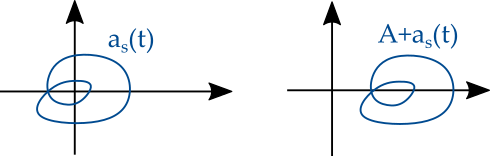
\includegraphics[width=8cm]{kk/figures/making min phase.png}
\caption{An SSB signal can be made minimum phase by adding a large enough subcarrier to it.}
\label{fig-make-min-phase}
\end{figure}
    
This also sheds some light on why these signals are called minimum phase: it is clear that the phase as seen from the origin of the signal on the right-hand side of Fig.~\ref{fig-make-min-phase} varies much less compared to the signal on the left-hand side.

In an actual telecommunication system, this extra subcarrier can be added either at the transmitter or at the receiver. Adding it at the transmitter reduces the complexity of the receiver, but requires sending a lot of power through the fibre, which can trigger nonlinear effects.

Finally, note that when you hear the term 'minimum phase' in the wild, it's typically used to refer to minimum-phase systems characterised by a certain transfer function. Here, we're talking about minimum-phase signals, which is slightly different. 

\hl{TODO: Jupyter notebook}

\pagebreak

\section{The Kramers-Kronig receiver}

Now it's finally time to describe the algorithm of the KK receiver in its full glory. To find the minimum-phase signal $a(t)$ from the intensity $|a(t)|^2$, we don't want to solve for the roots of the Z-extension, as that could be time-consuming. So, we're looking for another trick.

Recall our previous discussions about the Kramers-Kronig dispersion relations in Chapter~\ref{h:complex}: say we have a causal system, i.e. one with an impulse response that is zero for $t<0$. This translates in a complex frequency response $f(\omega)$ which is holomorphic in the upper half plane and which vanishes at infinite frequencies. Then, the imaginary part of the frequency response can be derived from its real part by Eq.~\ref{eq-KK-3}:

\begin{equation}
\Im f(\omega) = -\frac{1}{\pi} PV \int_{- \infty}^{\infty} \frac{\Re
    f(\omega')}{\omega'-\omega}d\omega'
\end{equation} 

Here, we are going to exchange the role of time and frequency. We start from an SSB signal, i.e. one with a frequency response that is zero for $\omega<0$. The complex envelope $a(t)$ is then holomorphic in the upper half plane and vanishes at $t=\infty$. Now, we have the following relationship between imaginary and real part of $a(t)$:

\begin{equation}
\Im a(t) = -\frac{1}{\pi} PV \int_{- \infty}^{\infty} \frac{\Re a(t')}{t'-t}dt'
\label{eq-kk-timedomain}
\end{equation} 

\noindent\marginnote[-2.7cm]{Eq.~\ref{eq-kk-timedomain} is valid for non-periodic signals, which have a Fourier transform rather than a Fourier series. We have been working with periodic signals so far, which obviously don't vanish at $t=\infty$. However, a similar-looking periodic variant of Eq.~\ref{eq-kk-timedomain} exists. We are going to sweep that technicality under the rug in what follows.}

Note that this equation is valid for all SSB signals, i.e. the signal does not necessarily have to be minimum phase.

Being able to derive the imaginary part from the real part of a signal is entertaining, but not really what we're after. We'd like to derive the phase from the amplitude instead.

\begin{cue}
If you write $a(t)=\left|a(t)\right| e^{j \phi(t)}$, can you construct a new function where the real and the imaginary part are related to $\left|a(t)\right|$ and $\phi(t)$?     
\end{cue}

This is achieved by introducing a new function:

\begin{equation}
L(t) = \ln\left(a(t)\right) = \ln \left( \left|a(t)\right| \right)+ j \phi(t)
\end{equation}

\pagebreak

\begin{cue}
At this point you're probably tempted to rush back and plug $L(t)$ into Eq.~\ref{eq-kk-timedomain} to derive the phase from the amplitude measurement. Why is this understandable urge premature?
\end{cue}

Remember that Eq.~\ref{eq-kk-timedomain} only holds for SSB signals. $a(t)$ is such a signal, but at the moment, we have no reason to assume that $\ln\left(a(t)\right)$ is SSB as well. However, this is where the minimum-phase property comes to the rescue, which is a piece of information we haven't relied on so far.

\begin{exer}
% difficulty: hard
By expanding $\ln(a(t))$ in a Fourier series and writing the Fourier coefficients as a contour integral over the unit circle, show that $\ln(a(t))$ has no negative frequencies. Is this still a band-limited signal?
\begin{hnt}
$l_k=-\frac{j}{2\pi} \oint_C \ln\left(\mathcal{Z}_a(z)\right) z^{-k-1} dz $
\end{hnt}
\end{exer}

Let's now summarise the recipe of the KK receiver. Start by creating an SSB signal, i.e. one which only contains frequencies to the right of a subcarrier.  Make the amplitude of the subcarrier large enough to end up with a minimum-phase signal. Perform an intensity measurement of this signal and figure out $\left|a(t)\right|$. Finally, recover the phase by performing the following calculation:

\begin{equation}
\phi(t) = -\frac{1}{\pi} PV \int_{-\infty}^{\infty} \frac{\ln \left( \left|a(t')\right| \right)}{t'-t}dt'
\label{eq-kk-timedomain-log}
\end{equation} 

The good news is that we only need a single photodiode as opposed to e.g. four. The bad news is that we require quite some postprocessing in the digital electronic domain. Depending on the requirements in terms of cost and power consumption of your application, that could be a valid trade-off.

\begin{exer}
% difficulty: hard
Would a telecommunication link based on maximum-phase signals work?
\end{exer} 

\section*{Review questions}

\begin{itemize}
\item What is the complex envelope of a signal?
\item When is a signal single-sideband? When minimum phase?
\item What is the winding number of a contour?
\item What is the logarithmic derivative?
\item What is the argument principle?  
\end{itemize}